\documentclass{beamer} 
\usepackage{amsmath,amsthm}
\usepackage{graphicx,microtype,parskip}
\usepackage{caption,subcaption,multirow}
\usepackage{attrib}

\frenchspacing

\usetheme{default}
\usecolortheme{whale}

\setbeamertemplate{navigation symbols}{}

\setbeamercolor{title}{fg=blue,bg=white}

\setbeamercolor{block title}{fg=white,bg=gray}
\setbeamercolor{block body}{fg=black,bg=lightgray}

\setbeamercolor{block title alerted}{fg=white,bg=darkgray}
\setbeamercolor{block body alerted}{fg=black,bg=lightgray}

\setbeamertemplate{footline} {
  \hbox{\begin{beamercolorbox}[wd=1\paperwidth,ht=2.25ex,dp=1ex,right]{framenumber}%
    \usebeamerfont{framenumber}\insertframenumber{} / \inserttotalframenumber\hspace*{2ex}
  \end{beamercolorbox}}%
  \vskip0pt%
}

\AtBeginSection[]
{
  \begin{frame}
    \tableofcontents[currentsection]
  \end{frame}
}


\title{Remodeling the fossil record}
\subtitle{analysis of emergent evolutionary and ecological patterns}
\author{Peter D Smits}
\institute{Committee on Evolutionary Biology, University of Chicago}
%\titlegraphic{
  %
\includegraphics[width=2.75cm,height=2.75cm,keepaspectratio=true]{figure/paleodb}
  %\hspace*{0.35\paperwidth}
  %
\includegraphics[width=2cm,height=2cm,keepaspectratio=true]{figure/chicago}
%}
\date{}

\begin{document}

\begin{frame}
  \maketitle
\end{frame}

\begin{frame}
  \tableofcontents
\end{frame}

\section{Macroevolution and macroecology}

\begin{frame}
  levels of organisation and emergence
  % i'm sure there is a compelling image that could be used here
  %   cells in tissue, tissue in organs, organs in organism, organism in population, etc.
\end{frame}

\begin{frame}
  \begin{definition}
    \begin{itemize}
      \item Macroevolution: study of patterns which emerge when considering the evolutionary history of multiple species.
      \item Macroecology: study of patterns which emerge when considering the ecology of multiple species.
      \item both in time and space
    \end{itemize}
  \end{definition}
\end{frame}

\begin{frame}
  trait: identifiable property of an organism

  species trait: idetifiable property of the entire species

  functional trait: class of traits describing interaction with environment
\end{frame}

\begin{frame}
  \frametitle{Species selection}

  \begin{block}{Rabosky and McCune 2010 \em{TREE}}
    \begin{quote}
      Species selection is the outcome of heritable variation in speciation and extinction rates among taxa.
    \end{quote}
  \end{block}

  \begin{itemize}
    \item avoids selection versus sorting
    \item avoids strict species selection vs effect macroevolution
    \item no operational structure
      \begin{itemize}
        \item species inherit traits
        \item traits affect fitness
      \end{itemize}
  \end{itemize}
\end{frame}

\begin{frame}
  \frametitle{Species fitness}

  \begin{definition}
    Expected time till extinction.
  \end{definition}
  
  \footnotesize{\attrib{Cooper 1984 \textit{J. Theoretical Biology}}} 

  \begin{itemize}
    \item \alert{logic:} if more fit, more likely to be present
    \item distribution based definition (population)
    \item other definitions can be derived, just expand definition of extinction
      \begin{itemize}
        \item lines-of-descent 
      \end{itemize}
  \end{itemize}

\end{frame}

\begin{frame}
%  \begin{block}{Extinction}
%    \begin{quote}
%      Population decline maybe a common cause of \dots extinction, but organisms never die from population decline, and population decline is never caused by organismal death alone \dots It's the relative balance between birth, death, and lifespan of organisms that determines \dots extinction. 
%    \end{quote}
%  \end{block}
%  
%  \small{\attrib{Simpson 2016 \em{bioRxiv}}}
\end{frame}

\begin{frame}
  \begin{alertblock}{Law of Constant Extinction}
    Extinction risk, in a given adaptive zone, is taxon--age independent.
  \end{alertblock}

  \small{\attrib{Van Valen 1973 \em{Evol. Theory}}}
\end{frame}

\begin{frame}
  \begin{block}{Survival of the unspecialized}
    \begin{quote}
      When related phyla die out \dots more specialized phyla tend to become extinct before less specialized. This phenomenon is also far from universal, but it is so common that it does deserve recognition as a rule or principle in evolutionary studies: \textbf{the rule of the survival of the relatively unspecialized.}
    \end{quote}
  \end{block}

  \small{\attrib{Simpson, 1944, \em{Tempo and Mode of Evolution}, p. 143}}
\end{frame}


\begin{frame}
  \frametitle{Species pool concept}

  \begin{center}
    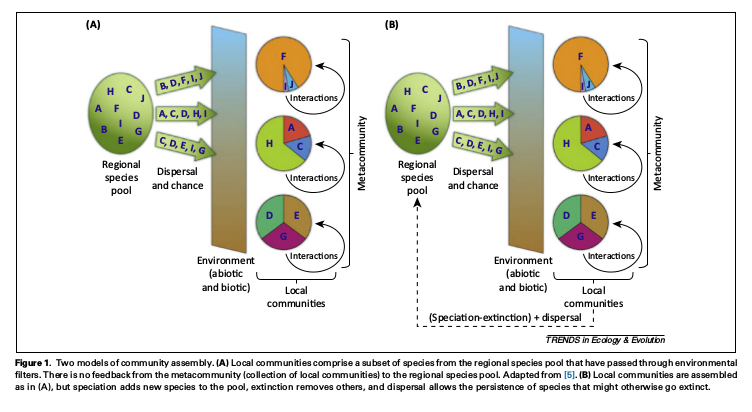
\includegraphics[height=0.8\textheight,width=\textwidth,keepaspectratio=true]{figure/schemske_pool}
  \end{center}

  \attrib{\footnotesize{Mittelbach and Schemske, 2015, \em{TREE}}}
\end{frame}

\begin{frame}
  functional composition of species pool
\end{frame}



\section{Structured data and modelling emergent patterns}

\begin{frame}
  \frametitle{Inference}

  Probability theory 

  Learning from incomplete information.

\end{frame}

\begin{frame}
  \frametitle{Inference devices and statistical models}

  statistical model as inference device

  engineering approach to analysis: building blocks used to create the device
\end{frame}

\begin{frame}
  \frametitle{Structured data in biology and paleontology}

  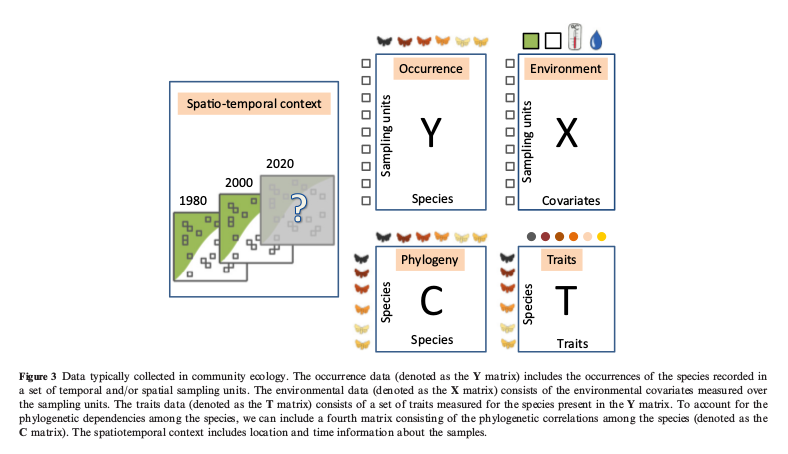
\includegraphics[width = \textwidth,height = 0.8\textheight,keepaspectratio = true]{figure/ovaskainen_data}

  \footnotesize{\attrib{Ovaskainen \textit{et al.} 2017 \textit{Ecology Letters}}}
\end{frame}

\begin{frame}
  \frametitle{Models of structured data}

  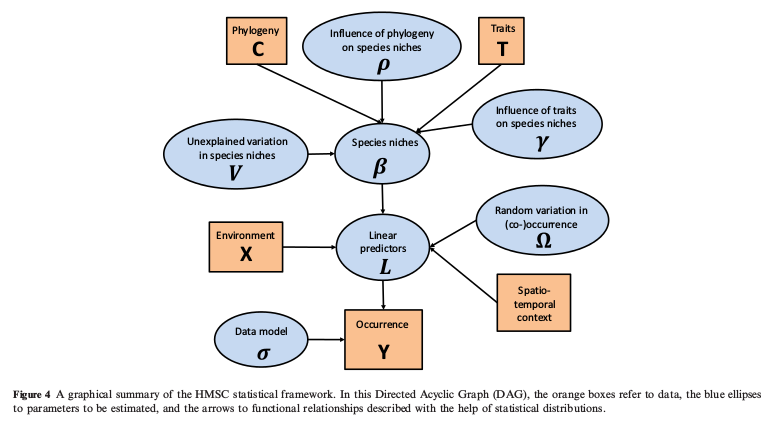
\includegraphics[width = \textwidth,height = 0.8\textheight,keepaspectratio = true]{figure/ovaskainen_dag}

  \footnotesize{\attrib{Ovaskainen \textit{et al.} 2017 \textit{Ecology Letters}}}
\end{frame}


\begin{frame}
  \frametitle{Models of macroevolution}

  birth-death for diversity

  Brownian motion for trait
\end{frame}


\begin{frame}
  \frametitle{Species distribution models}

  \begin{columns}
    \begin{column}{0.5\textwidth}
      \begin{block}{Goal}
        Understand relationship between species distribution in space (and time) as function of that species' environmental context or species trait values.
      \end{block}
    \end{column}
    \begin{column}{0.5\textwidth}
      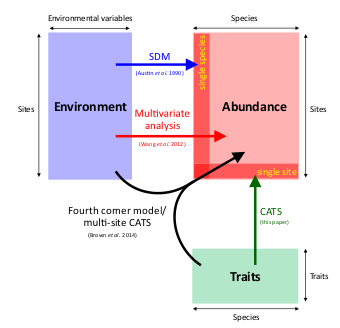
\includegraphics[width = \textwidth,height = 0.8\textheight,keepaspectratio = true]{figure/warton_corner_models}

      \footnotesize{\attrib{Warton \textit{et al.} 2015 \textit{Methods in Ecology and Evolution}}}
    \end{column}
  \end{columns}
\end{frame}


\begin{frame}
  \frametitle{Bayesian statistics}

  framework used throughout this dissertation

  flexible, expressive, intuitive

  using HMC and ADVI as implemented in Stan 
\end{frame}


\section{Patterns in survival}
\subsection{Background extinction and expected differences in species survival}

\begin{frame}
  \begin{block}{Motivating questions}
    \begin{itemize}
      \item \alert{How do mammal species traits affect extinction risk?}
        \begin{itemize}
          \item How do shared time of origination or evolutionary history relate to extinction risk?
        \end{itemize}
      \item How do my findings compare to current risk factors?
      \item Is species extinction risk age-independent?
    \end{itemize}
  \end{block}
\end{frame}

\begin{frame}
  Cenozoic mammals of North America
\end{frame}

\begin{frame}
  \frametitle{Relationship between range size and extinction risk}
  \begin{center}
    %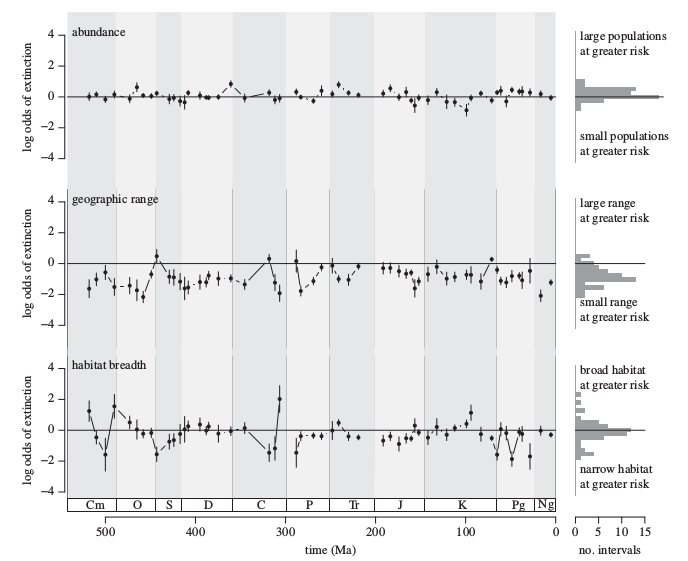
\includegraphics[width = \textwidth,height = 0.8\textheight,keepaspectratio = true]{figure/harnik_rarity}
  \end{center}

  \tiny{\attrib{Harnik and Simpson 2013 \textit{Proc B}}}
\end{frame}


\begin{frame}
  \frametitle{Hypotheses of effects of dietary category}
  \begin{center}
    %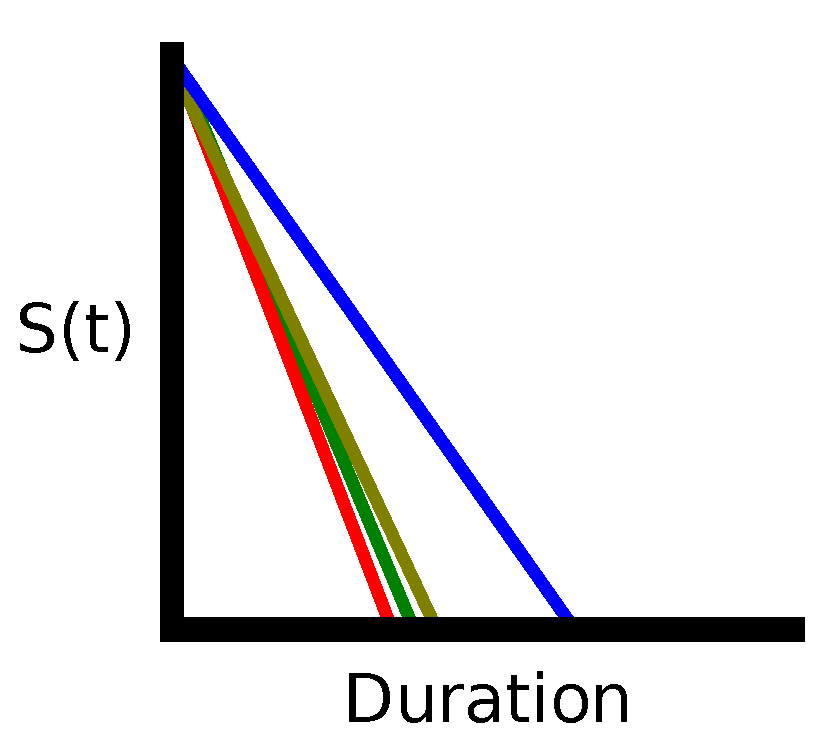
\includegraphics[width = \textwidth,height = 0.8\textheight,keepaspectratio = true]{figure/diet_survival}
  \end{center}
\end{frame}

\begin{frame}
  \frametitle{Hypotheses of effects of locomotor category}
  \begin{center}
    %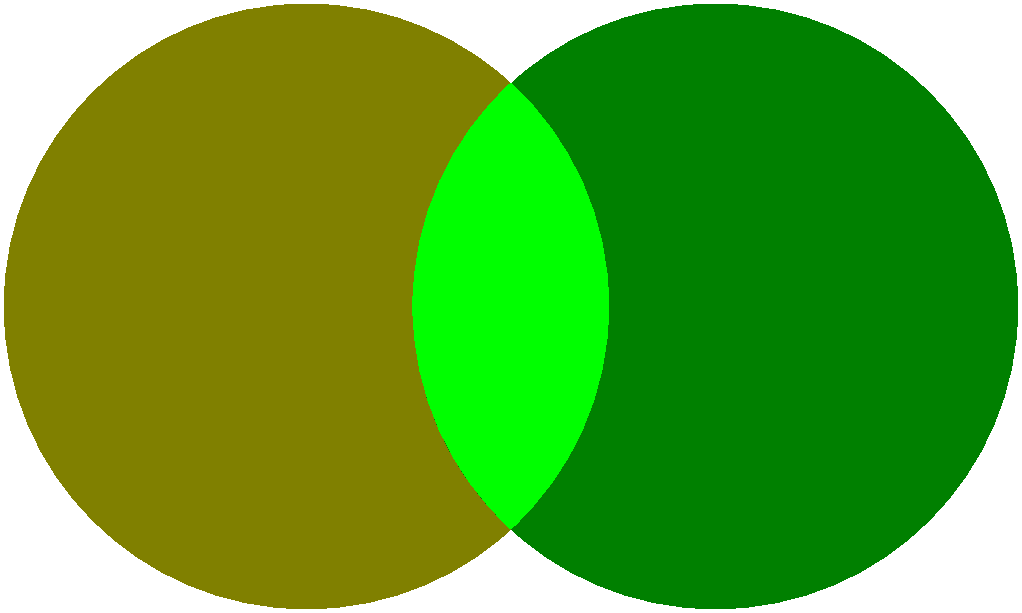
\includegraphics[width = \textwidth,height = 0.8\textheight,keepaspectratio = true]{figure/loco_initial}
  \end{center}
\end{frame}

\begin{frame}
  \frametitle{Hypotheses of effects of locomotor category}
  \begin{center}
    %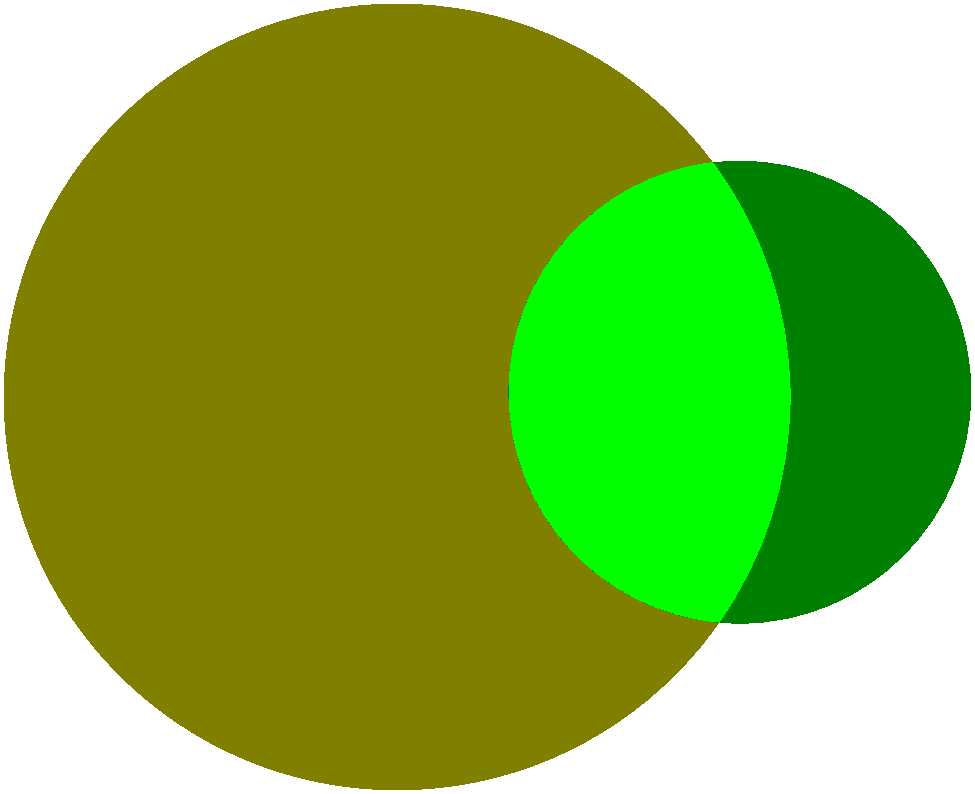
\includegraphics[width = \textwidth,height = 0.8\textheight,keepaspectratio = true]{figure/loco_later}
  \end{center}
\end{frame}

\begin{frame}
  \frametitle{Survival model diagram}
  \begin{center}
    %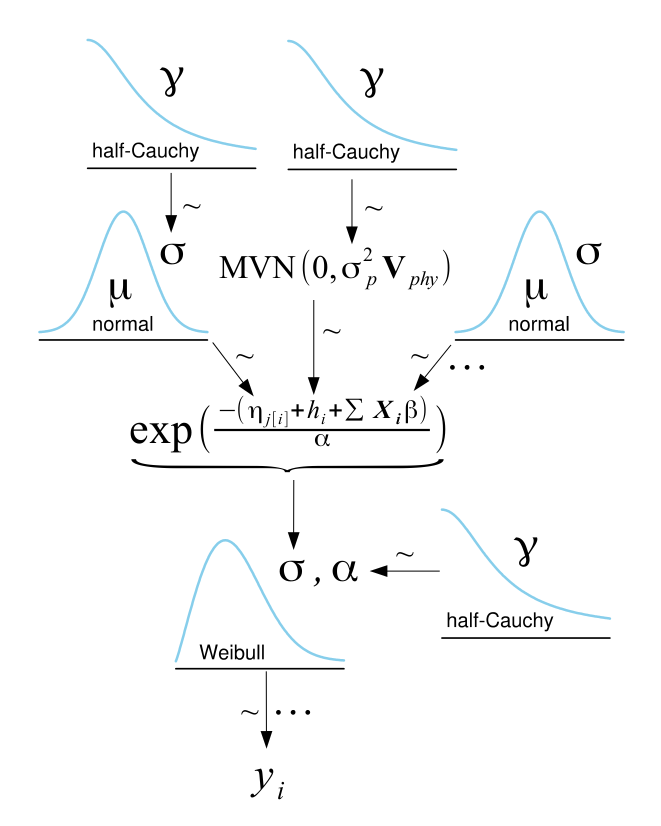
\includegraphics[height=0.8\textheight,keepaspectratio=true]{figure/mammal_model}
  \end{center}
\end{frame}

\begin{frame}
  \frametitle{Pattern of species survival under two models}

  %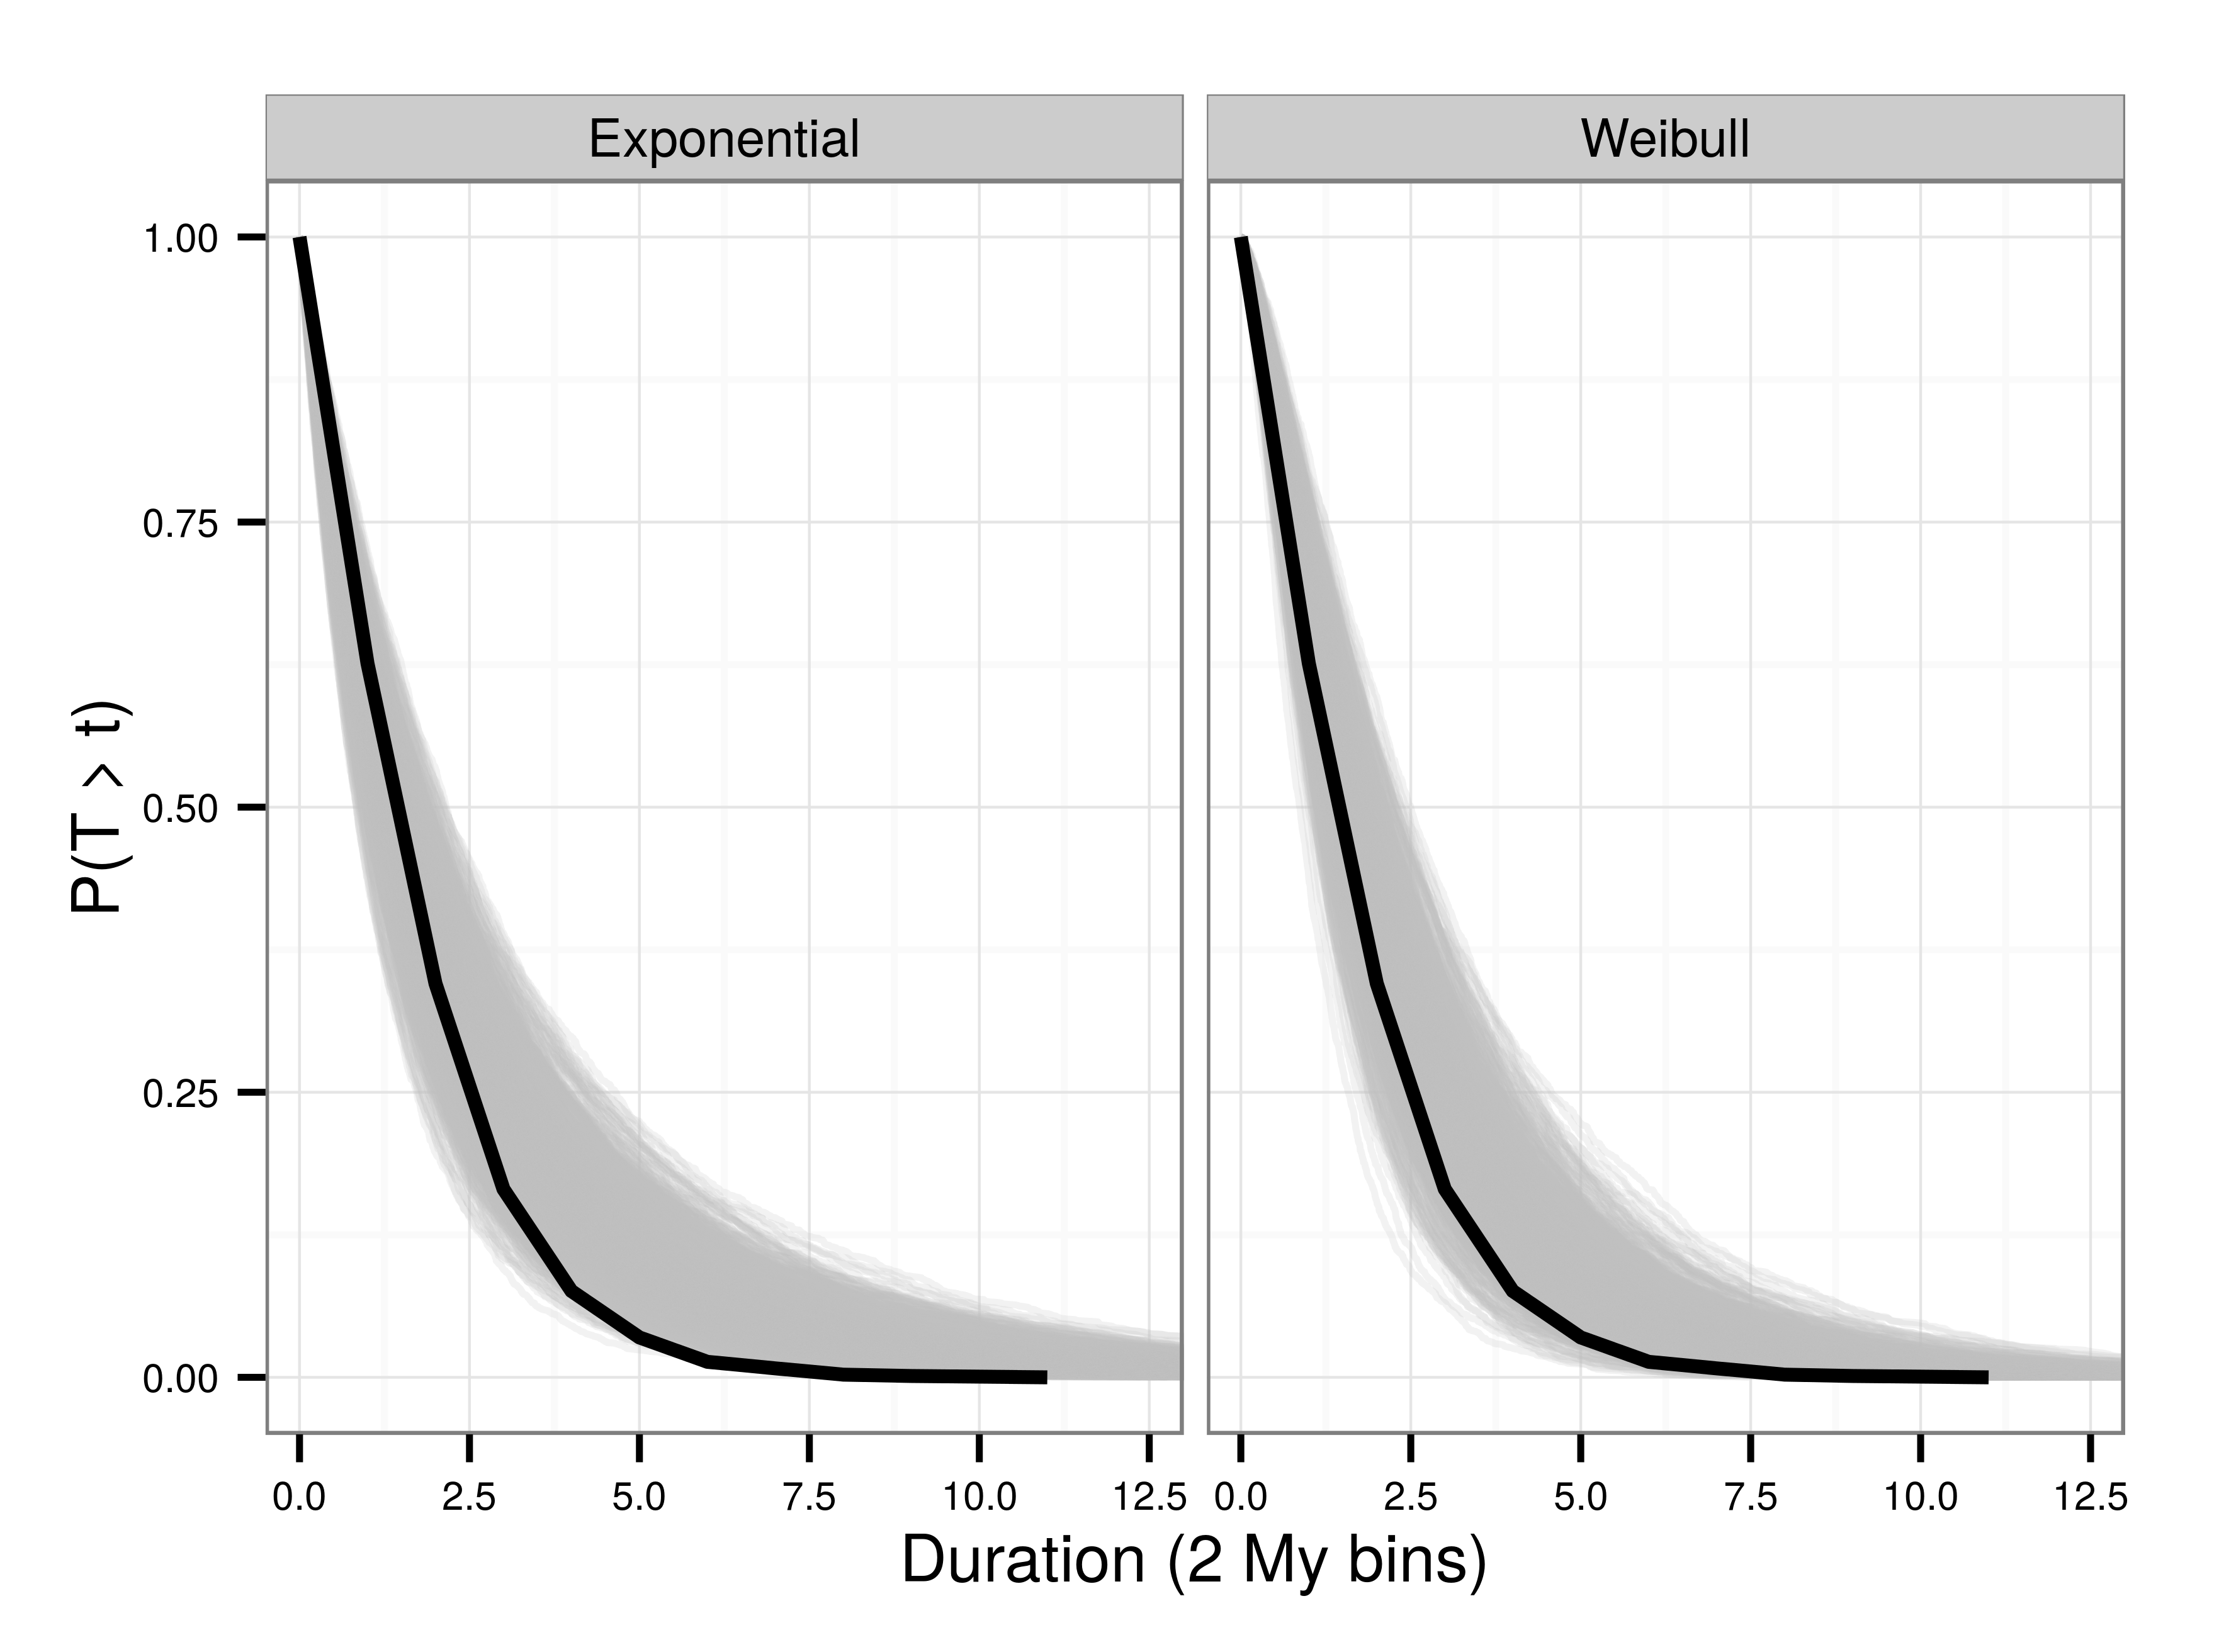
\includegraphics[height=0.8\textheight,keepaspectratio=true]{figure/survival_function_pres}
\end{frame}

\begin{frame}
  \frametitle{Effect of dietary category on extinction risk}

  %\includegraphics[height=0.8\textheight,keepaspectratio=true]{figure/diet_diff_est_pres}
\end{frame}

\begin{frame}
  \frametitle{Effect of locomotor category on extinction risk}

  %\includegraphics[height=0.8\textheight,keepaspectratio=true]{figure/loco_diff_est_pres}
\end{frame}

\begin{frame}
  \frametitle{Difference in risk between origination cohorts}

  %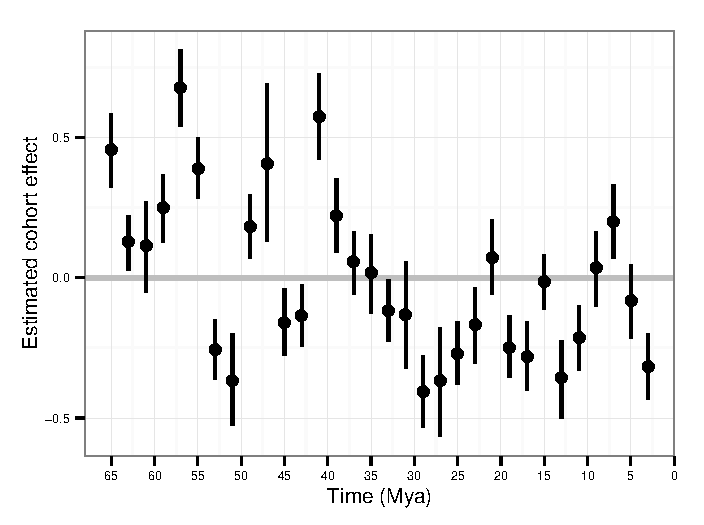
\includegraphics[height=0.8\textheight,keepaspectratio=true]{figure/cohort_est_pres}
\end{frame}

\begin{frame}
  \frametitle{Three sources of variance}

  %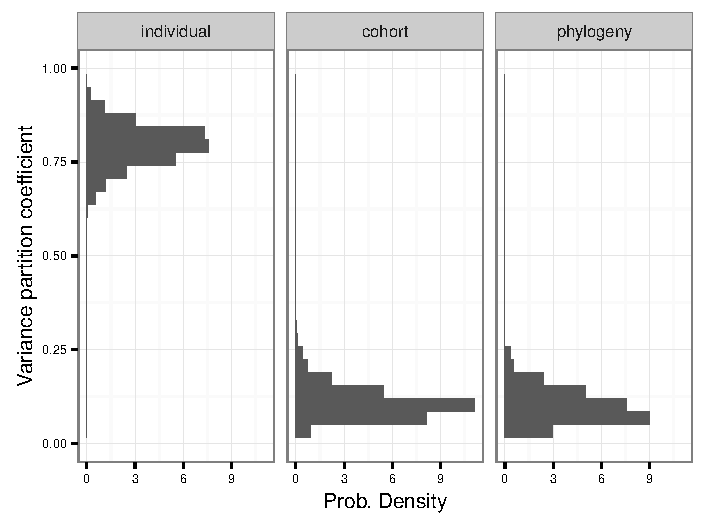
\includegraphics[height=0.8\textheight,keepaspectratio=true]{figure/variance_est_pres}
\end{frame}

\begin{frame}
  \begin{block}{Conclusions}
    \begin{itemize}
      \item Survival of the unspecialized as time-invariant generalization.
      \item Decrease in extinction risk with time.
        \begin{itemize}
          \item Both cohort/temporal and phylogenetic effect.
        \end{itemize}
      \item Some incongruence with risk factors in the Recent.
        \begin{itemize}
          \item e.g. effect of body size, trophic category, phylogenetic clustering.
        \end{itemize}
    \end{itemize}
  \end{block}
\end{frame}



\subsection{Interplay between extinction intensity and extinction selectivity}

\begin{frame}
  \begin{alertblock}{Observation}
    At K/Pg mass extinction, biological traits (except geographic range) have no effect on \alert{bivalve} taxonomic survival.

    \attrib{\footnotesize{Jablonski, 1986, \em{Science}}}
  \end{alertblock}
\end{frame}

\begin{frame}
  \begin{alertblock}{Questions and analysis}
    \begin{itemize}
      \item How do the effect of emergent traits on duration (\alert{extinction selectivity}) vary with expected duration (\alert{extinction intensity})?
      \item \textbf{Approach:} hierarchical Bayesian survival model; \\effect estimates vary with origination cohort; \\correlation btw effects modeled.
    \end{itemize}
  \end{alertblock}
\end{frame}

\begin{frame}
  \frametitle{Intensity and selectivity}
  \begin{center}
    %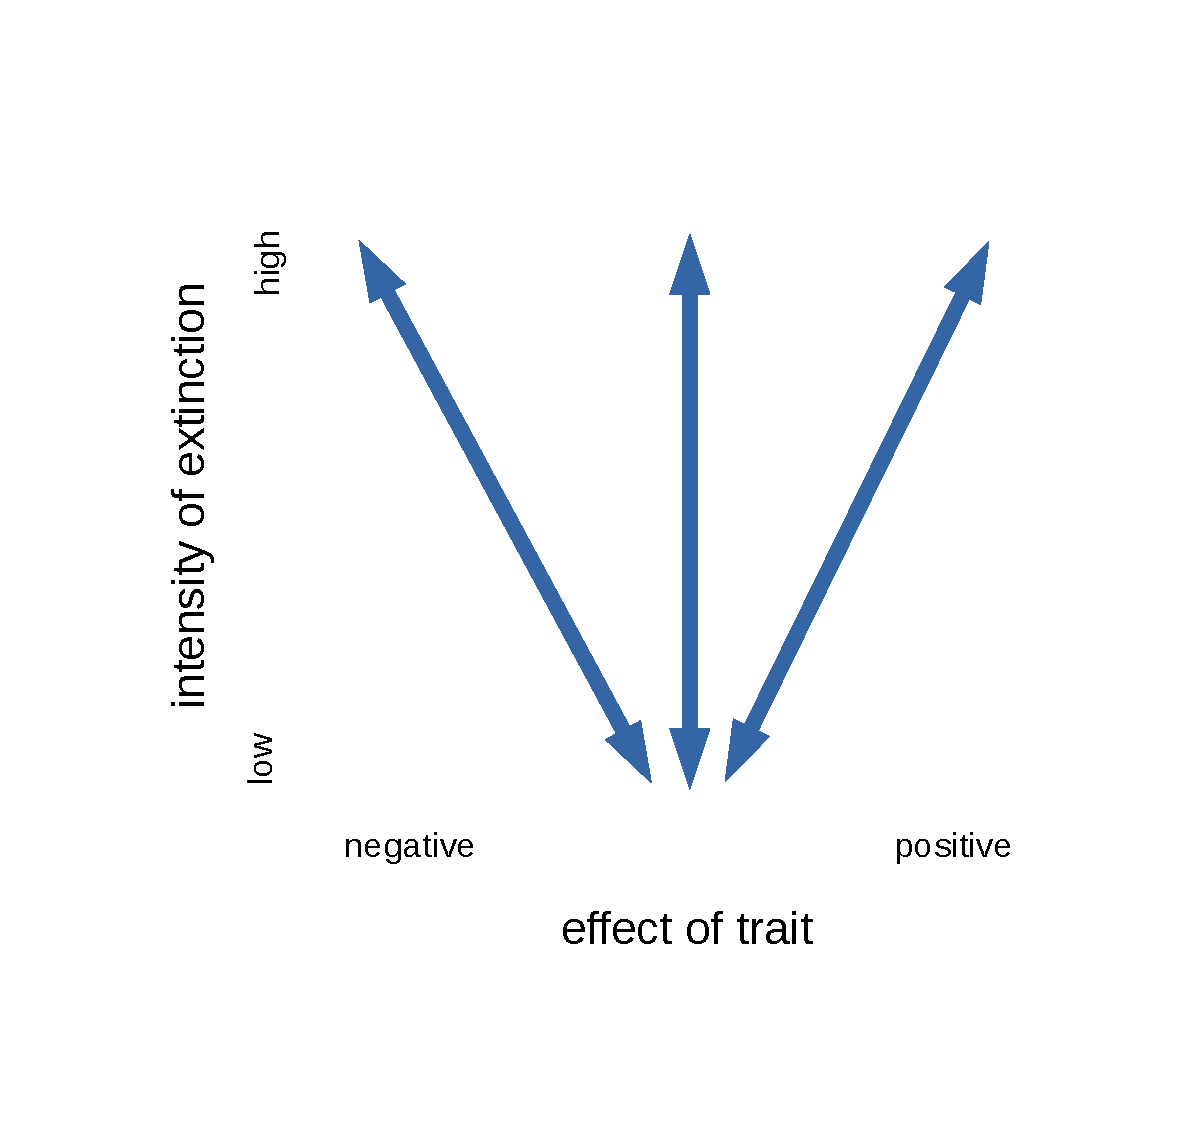
\includegraphics[width = \textwidth,height = 0.8\textheight,keepaspectratio = true]{figure/intensity_selectivity_base}
  \end{center}
\end{frame}

\begin{frame}
  \frametitle{Brachiopods}
  %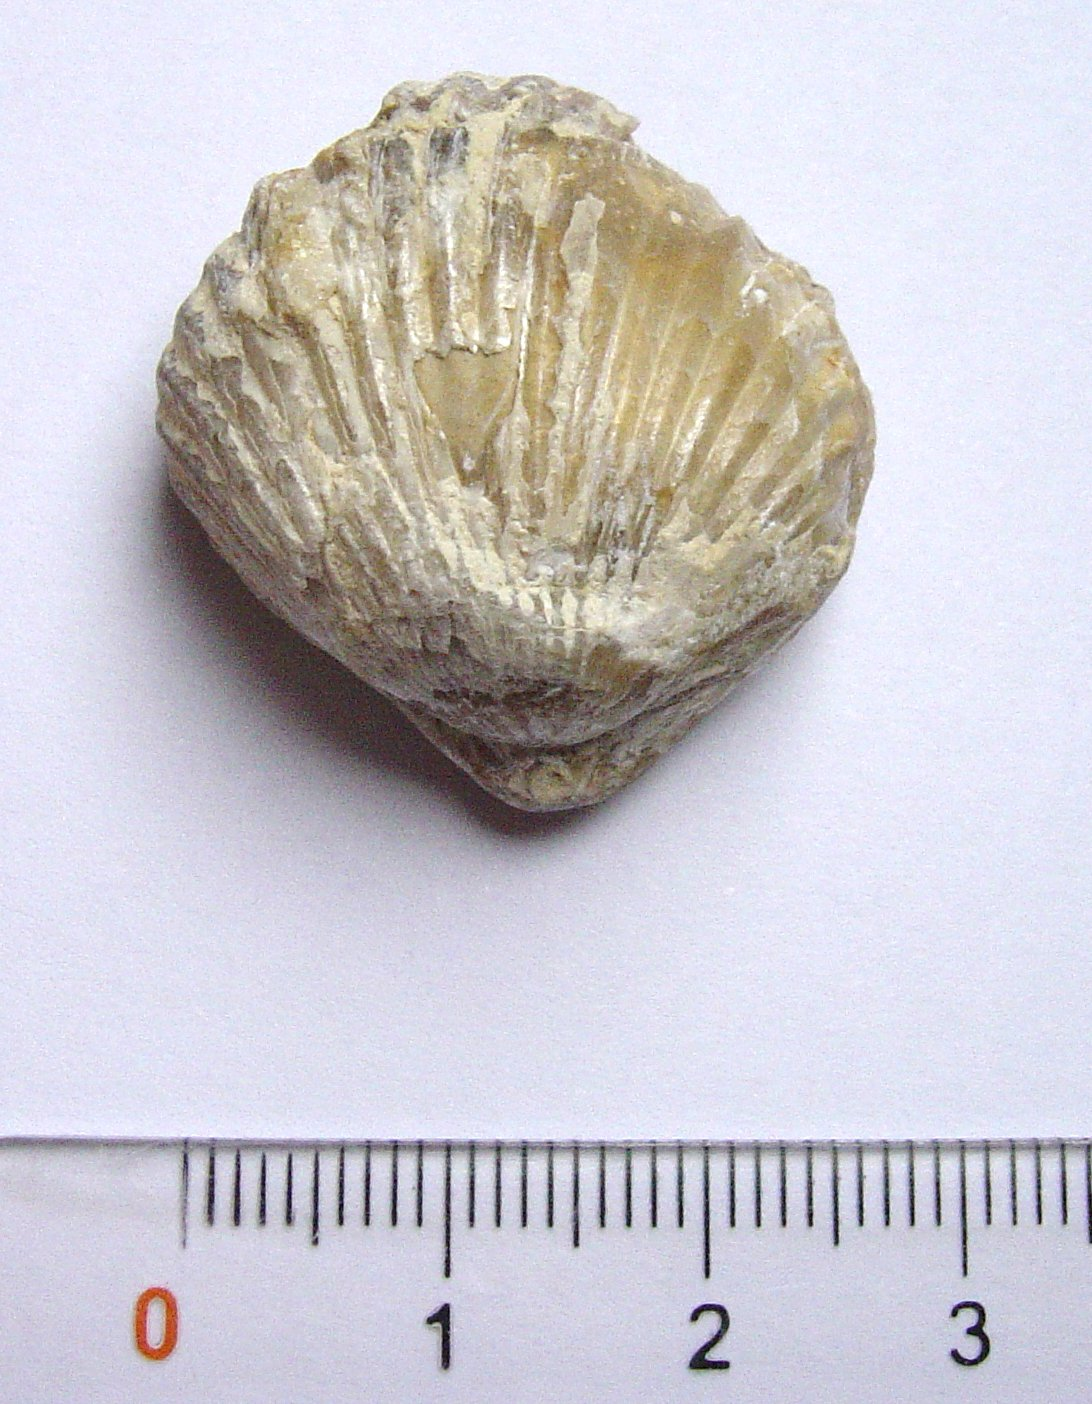
\includegraphics[width = 0.45\textwidth,height = 0.8\textheight,keepaspectratio = true]{figure/Brachiopod_fossil}
  %\includegraphics[width = 0.45\textwidth,height = 0.8\textheight,keepaspectratio = true]{figure/Burmirhynchionella_decorata_brachial_CRF}

  \footnotesize{\attrib{ComputerHotline, wikimedia CC BY 2.5; Dwergenpaartje, wikimedia CC BY-SA 3.0}}
\end{frame}

\begin{frame}
  \frametitle{Post-Cambrian Paleozoic brachiopod genera and covariates}
  \begin{itemize}
    \item time range approx. 488-252 Mya.
    \item stage as time unit; duration measured in stages (2-5 My each)
    \item multiple emergent traits analyzed; estimates vary by origination cohort
      \begin{itemize}
        \item geographic range
        \item body size
        \item environmental preference (v, v\(^2\))
      \end{itemize}
    \item gap statistic as measure of sampling {\footnotesize{(Foote and Raup 1996 \textit{Paleobio})}} \\imputed for taxa with short durations
  \end{itemize}
\end{frame}


\begin{frame}
  \frametitle{Hierarchical survival model}
  \begin{center}
    %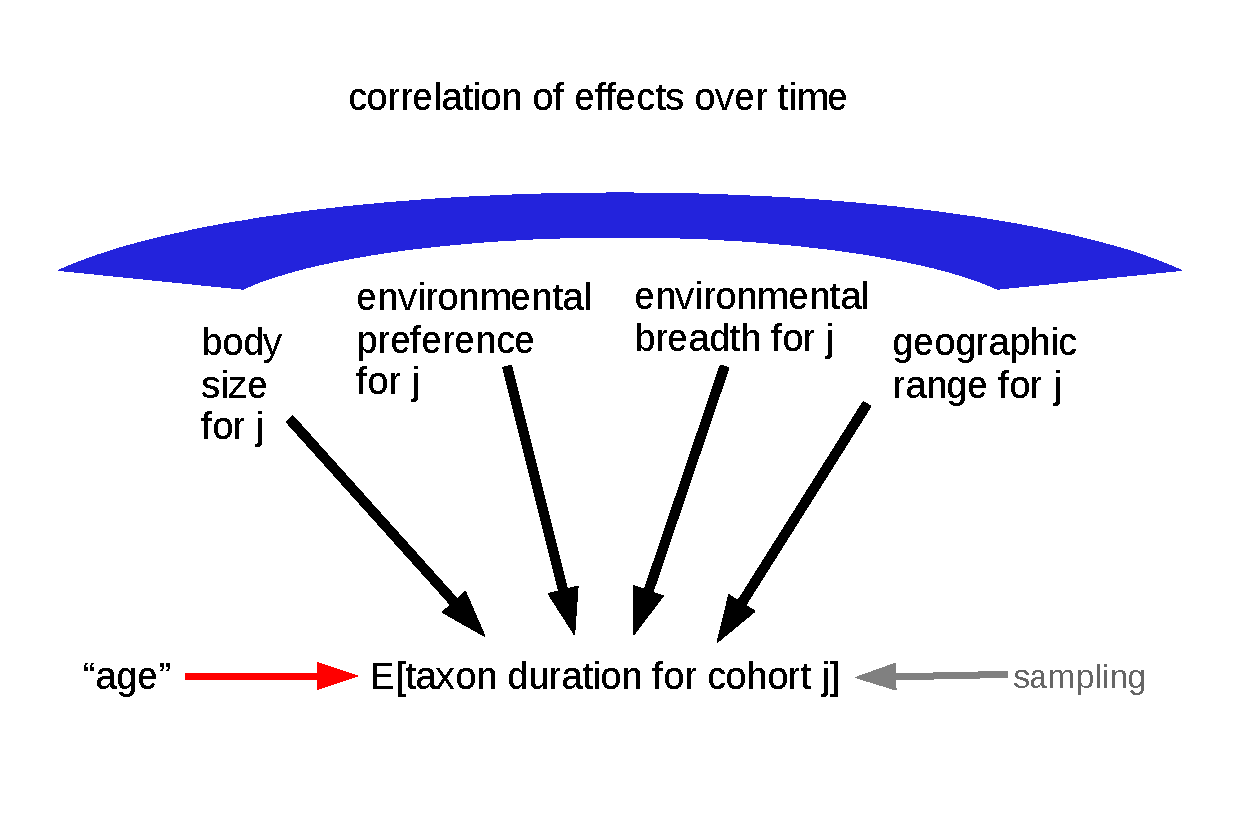
\includegraphics[width = \textwidth,height = 0.8\textheight,keepaspectratio = true]{figure/simple_model}
  \end{center}
\end{frame}

\begin{frame}
  \frametitle{Sampling statement for the joint posterior probability}
  \begin{columns}
    \begin{column}{0.5\textwidth}
      \begin{align*}
        y_{i, t} &\sim \text{Weibull}(\sigma_{i, t}, \alpha) \\
        \log(\sigma_{i, t}) &= \frac{X_{i}B_{j[i], t} + \delta s_{i}}{\alpha} \\
        B_{j} &\sim \text{MVN}(\mu, \Sigma) \\
        \Sigma &= \text{diag}(\tau) \Omega \text{diag}(\tau) \\
        s_{i} &\sim \text{Beta}(\phi_{i}, \lambda) \\
        \phi_{i} &= \text{logit}^{-1}(W_{i}\gamma) \\
      \end{align*}
    \end{column}
    \begin{column}{0.5\textwidth}
      \begin{align*}
        \mu_{intensity} &\sim \mathcal{N}(0, 5) \\
        \mu_{range} &\sim \mathcal{N}(-1, 1) \\
        \mu_{env pref} &\sim \mathcal{N}(0, 1) \\
        \mu_{env curve} &\sim \mathcal{N}(1, 1) \\
        \mu_{size} &\sim \mathcal{N}(0, 1) \\
        \delta &\sim \mathcal{N}(0, 1) \\
        \tau &\sim \text{C}^{+}(1) \\
        \Omega &\sim \text{LKJ}(1) \\
        \lambda &\sim \text{Pareto}(0.1, 1.5) \\
        \gamma &\sim \mathcal{N}(0, 1) \\
      \end{align*}
    \end{column}
  \end{columns}

  \scriptsize{Note: Calculation of log probability of right and left censored observations is modified from the above}
\end{frame}



\begin{frame}
  \frametitle{Model adequacy}
  \begin{columns}
    \begin{column}{0.5\textwidth}
      \begin{center}
        %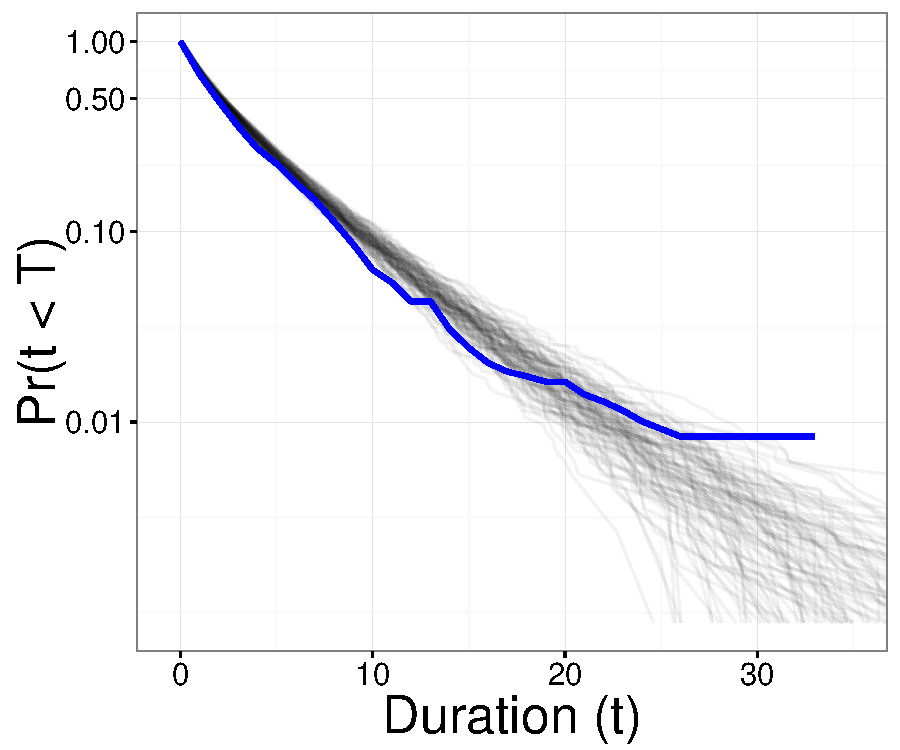
\includegraphics[width=\textwidth,height=0.8\textheight,keepaspectratio=true]{figure/survival_curves}
      \end{center}
    \end{column}
    \begin{column}{0.5\textwidth}
      \begin{center}
        %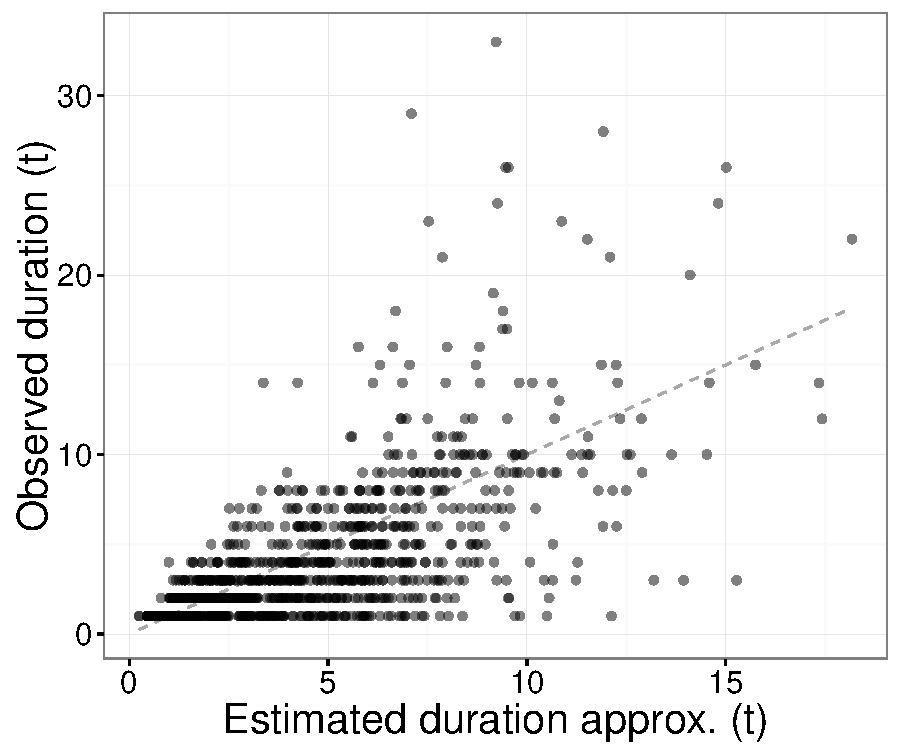
\includegraphics[width=\textwidth,height=0.8\textheight,keepaspectratio=true]{figure/shotgun}
      \end{center}
    \end{column}
  \end{columns}
\end{frame}

\begin{frame}
  \frametitle{Variation in trait effects between cohorts}

  \begin{center}
    %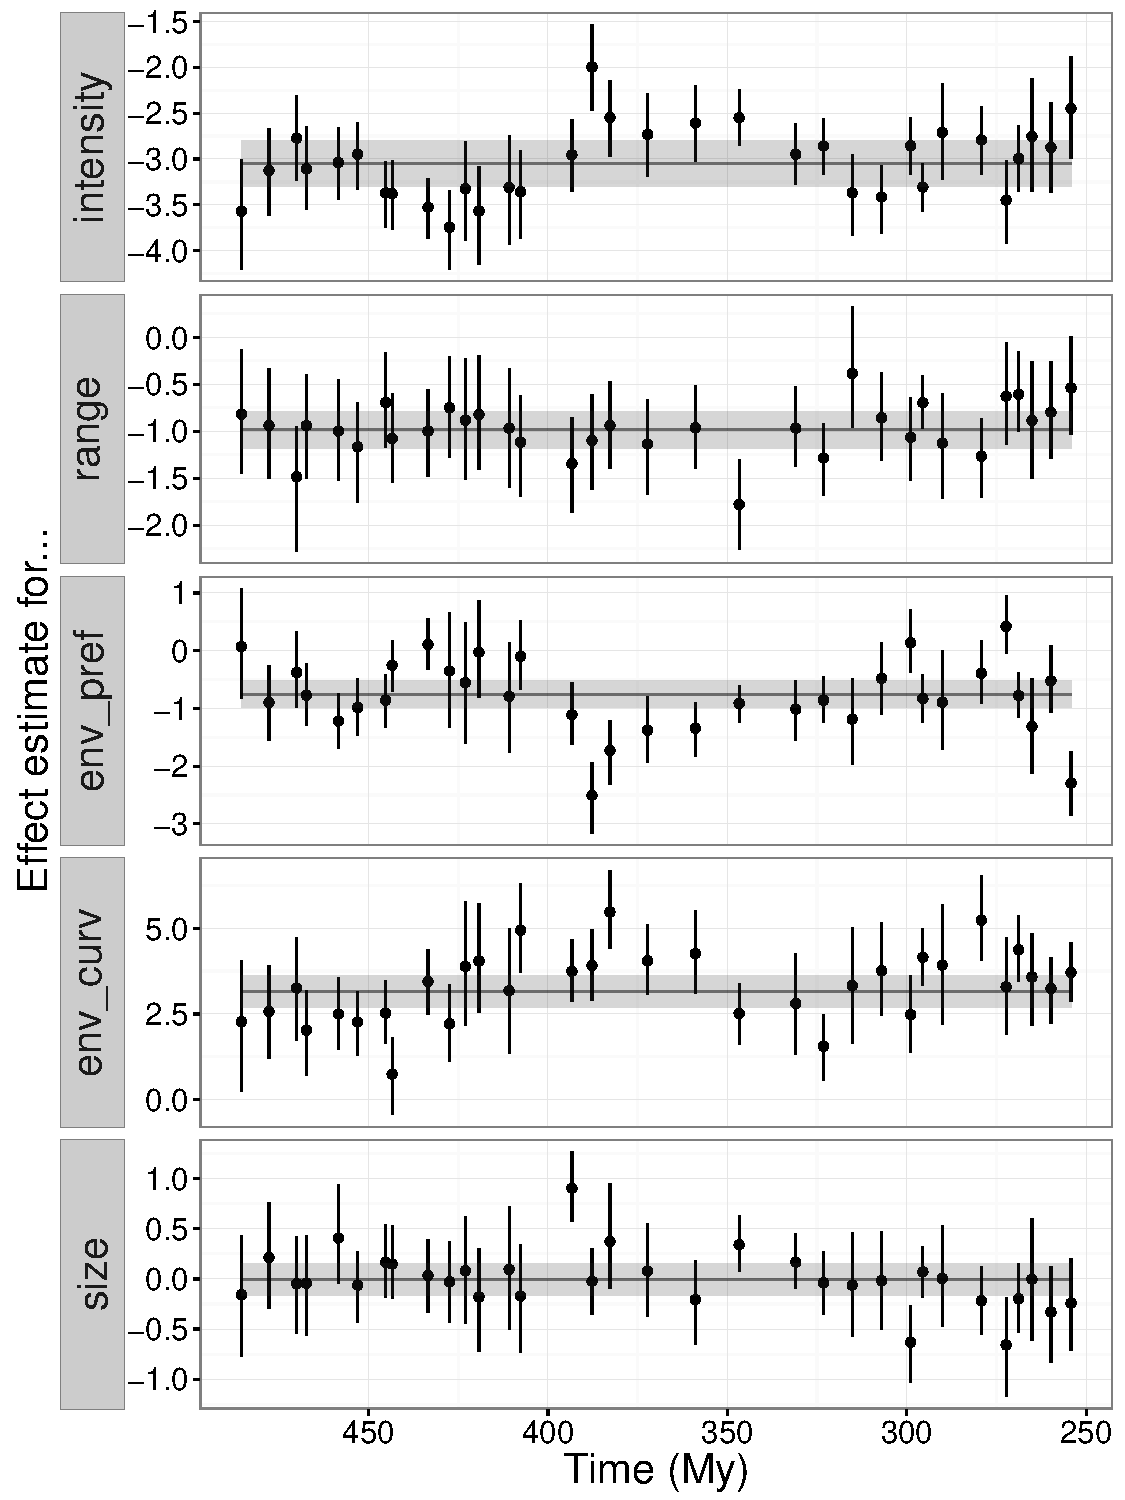
\includegraphics[width = \textwidth,height = 0.8\textheight,keepaspectratio = true]{figure/cohort_series}
  \end{center}
\end{frame}

\begin{frame}
  \frametitle{Overall effect of environmental preference}

  \begin{center}
    %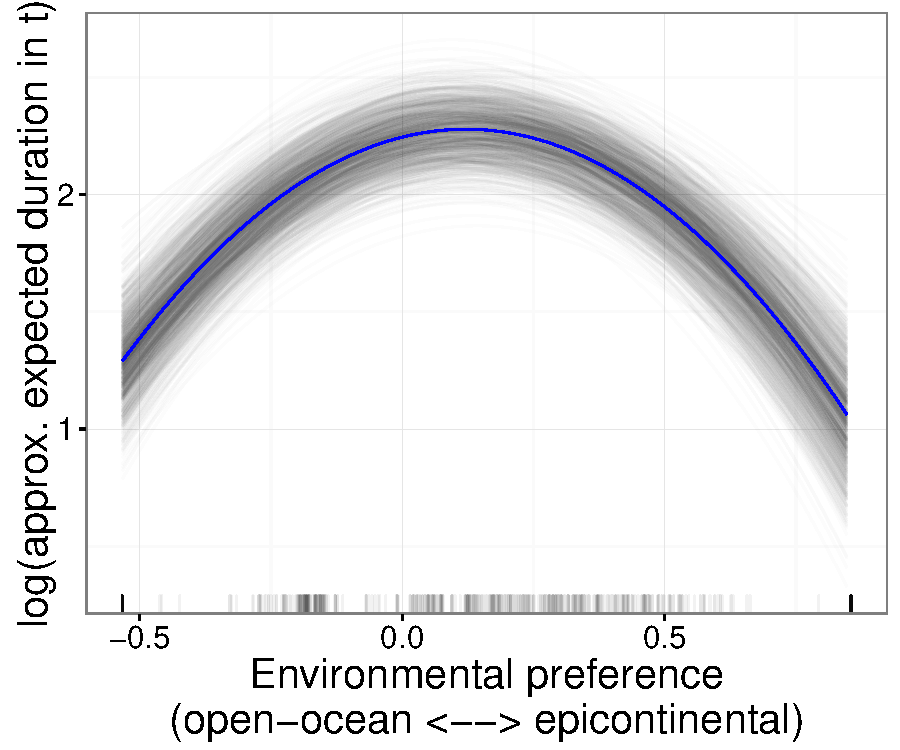
\includegraphics[width = \textwidth,height = 0.8\textheight,keepaspectratio = true]{figure/env_effect}
  \end{center}
\end{frame}

\begin{frame}
  \frametitle{Change in effect of environment between cohorts}

  \begin{center}
    %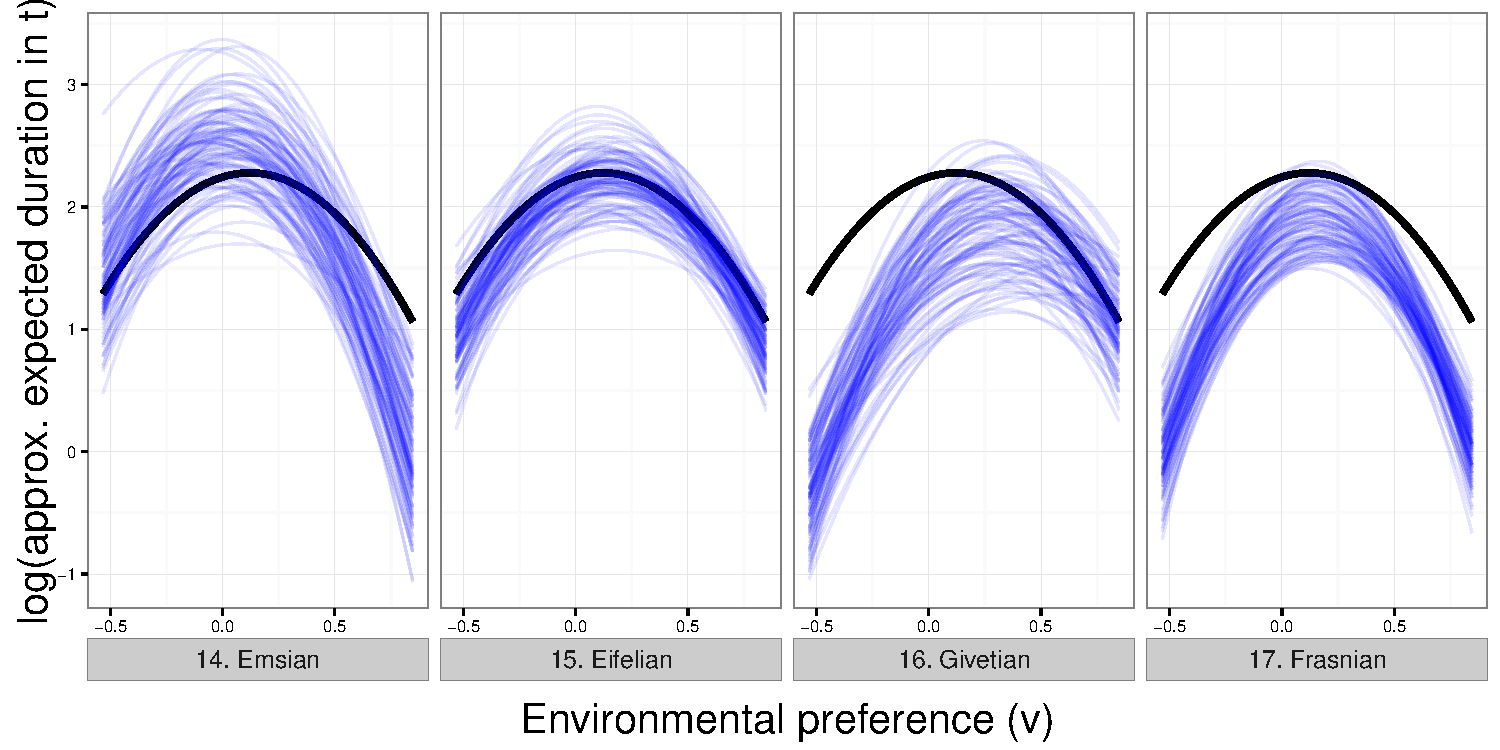
\includegraphics[width = \textwidth,height = 0.8\textheight,keepaspectratio = true]{figure/env_cohort_short}
  \end{center}
\end{frame}

\begin{frame}
  \frametitle{Change in effect of environment between cohorts}

  \begin{center}
    %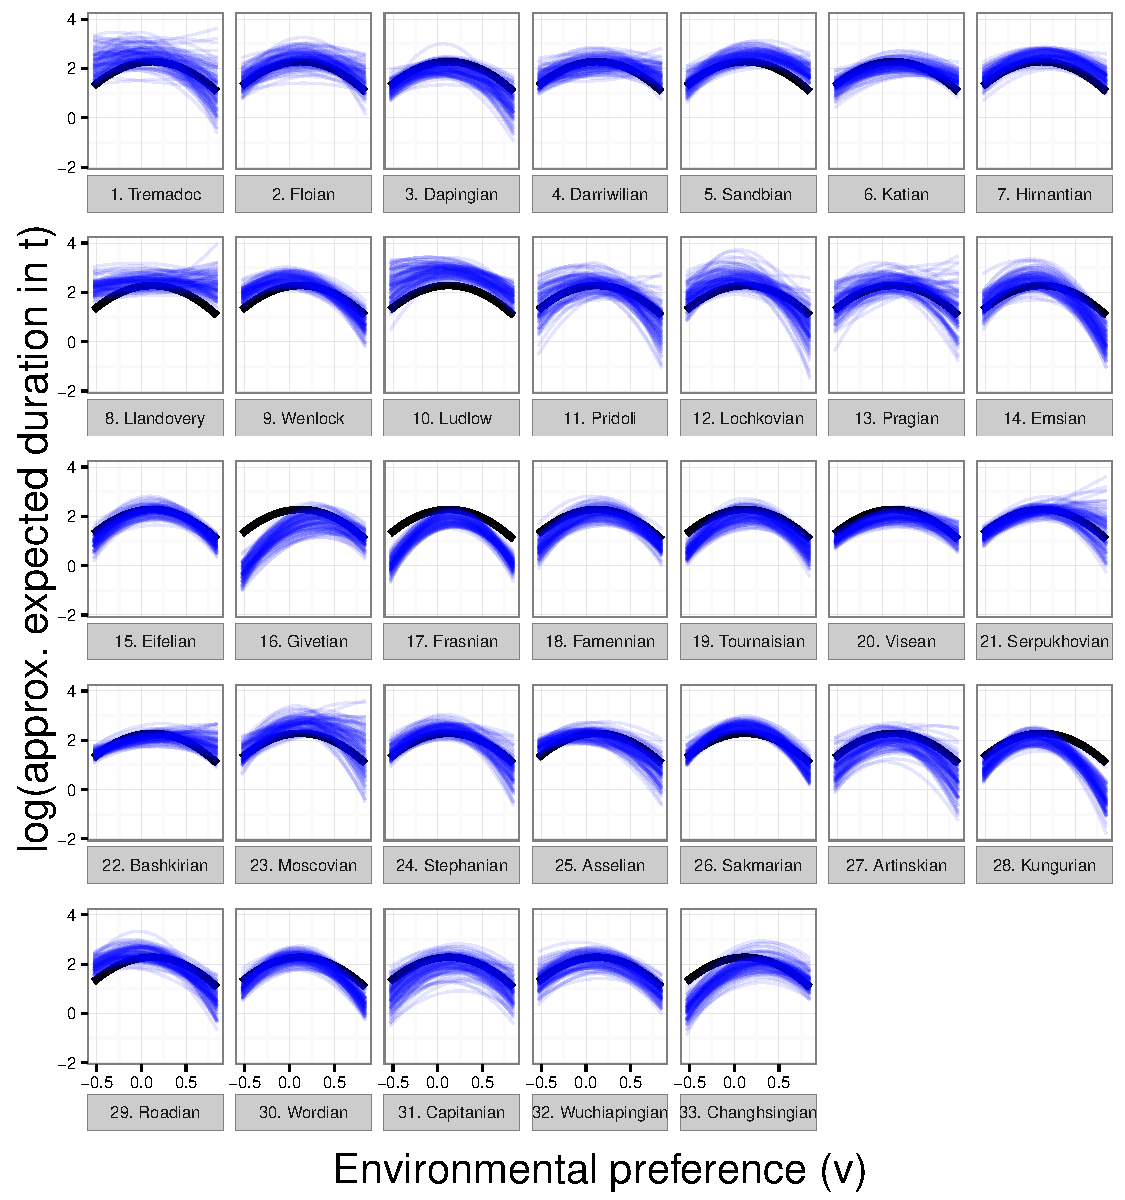
\includegraphics[width = 0.8\textwidth,height = 0.8\textheight,keepaspectratio = true]{figure/env_cohort}
  \end{center}
\end{frame}

\begin{frame}
  \frametitle{Correlation of effects between cohorts}

  \begin{center}
    %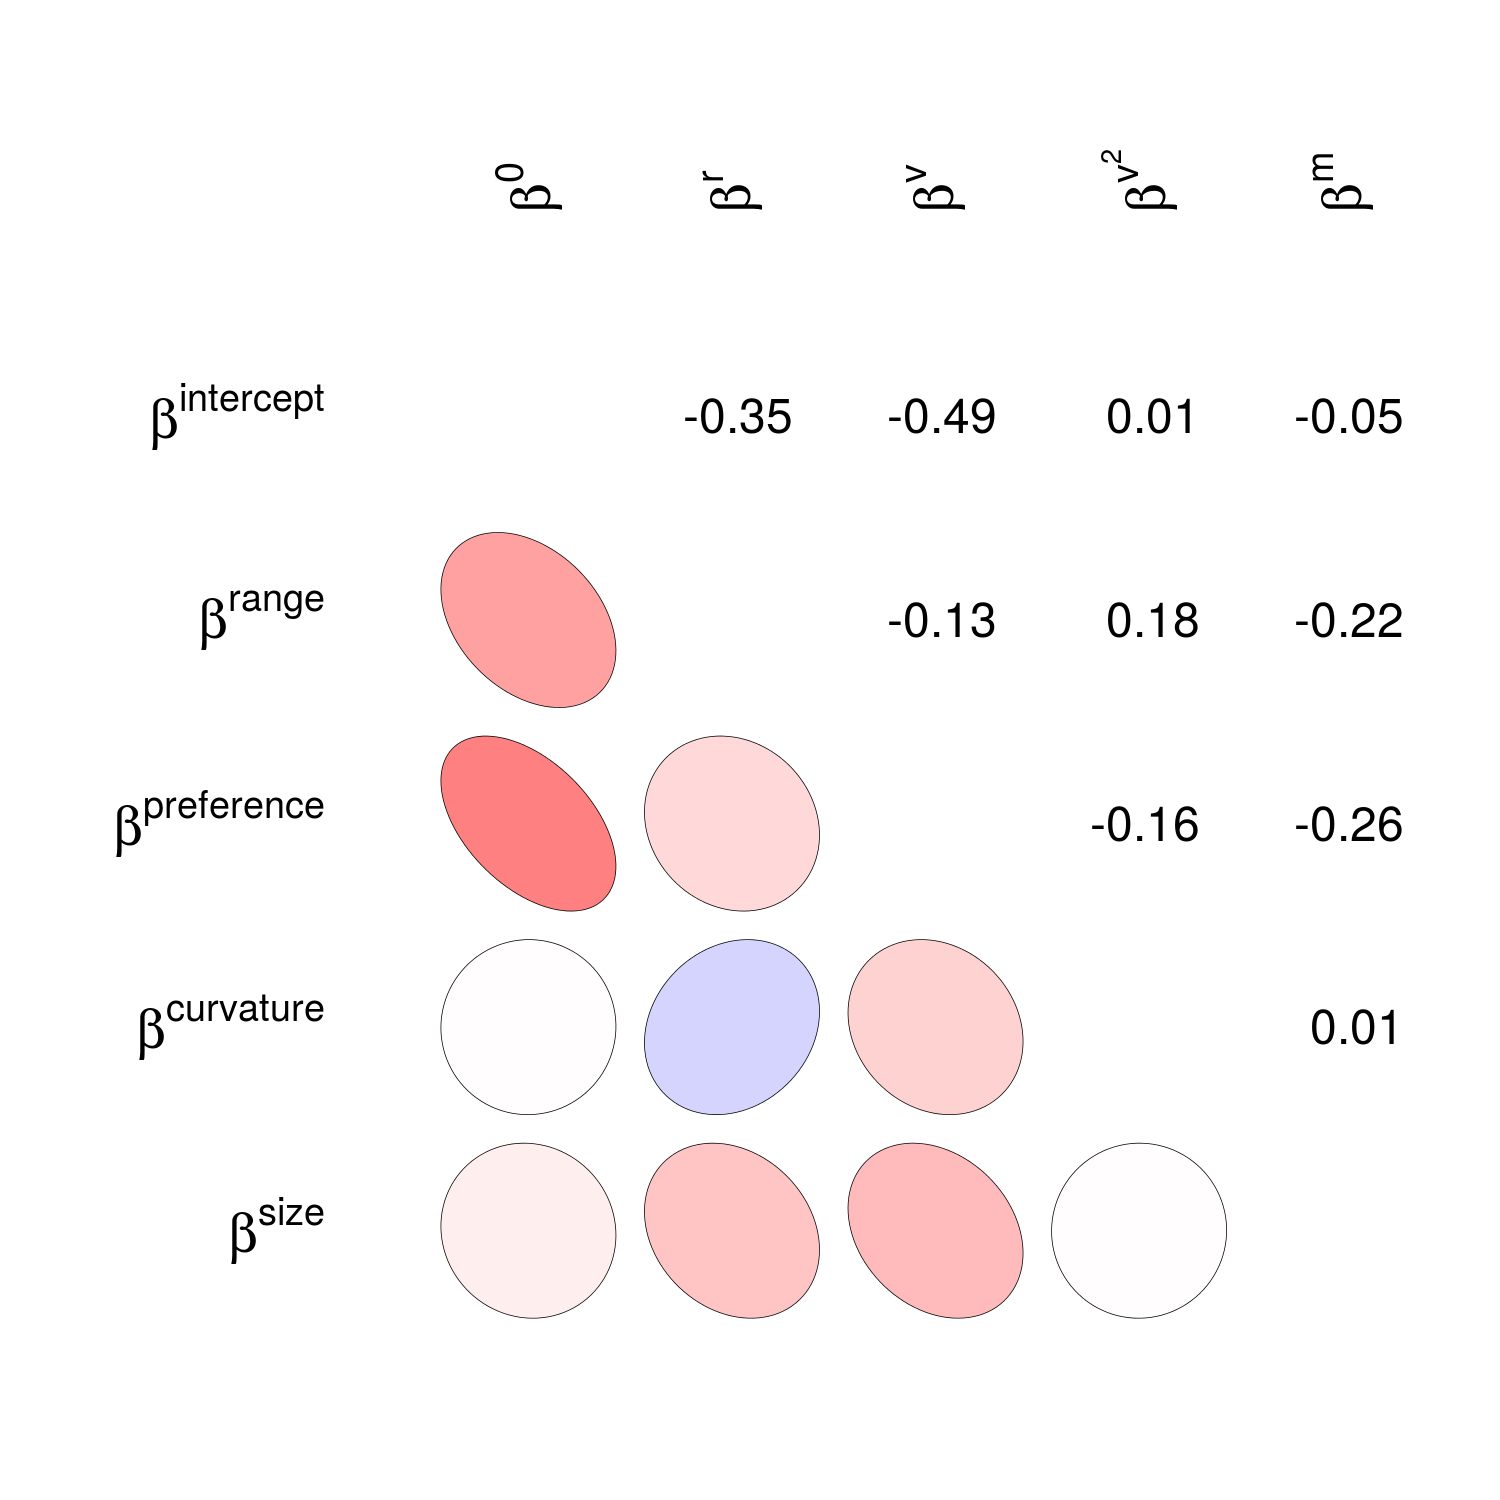
\includegraphics[width = \textwidth,height = 0.9\textheight,keepaspectratio = true]{figure/wei_cor_heatmap}
  \end{center}
\end{frame}

\begin{frame}
  \begin{block}{Effect summary}
    \begin{itemize}
      \item Effect of geographic range consistent with prior expectations; low variance.
      \item No effect of body size; low variance.
      \item Epicontinental environmental preference slightly favored on averaged; high variance. 
      \item Strong support for survival of unspecialized as generalization wrt environmental preference; medium variance.
    \end{itemize}
  \end{block}
\end{frame}

\begin{frame}
  \begin{alertblock}{Macroevolutionary process}
    \begin{itemize}
      \item Magnitude of effect of geographic range and environmental preference increase with extinction intensity.
      \item As extinction risk decreases, the differences between taxa matter less.
    \end{itemize}
  \end{alertblock}
\end{frame}



\section{Patterns in functional diversity}
\subsection{Mammal species pool functional composition}


\begin{frame}
  \begin{center}
    %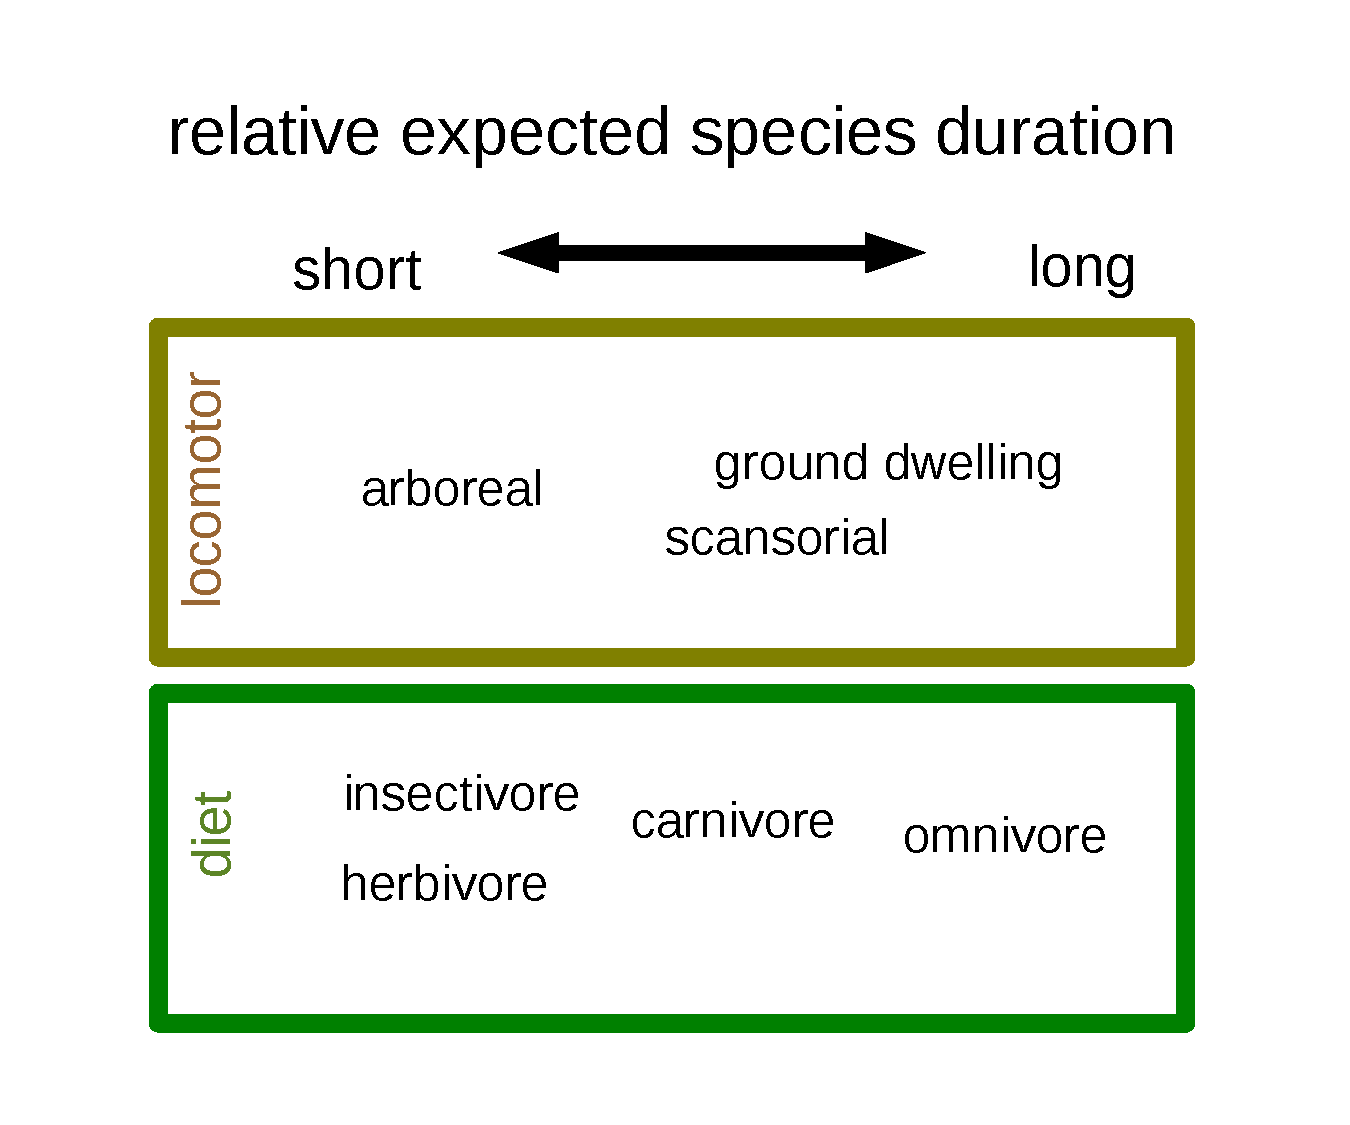
\includegraphics[height=0.8\textheight,width=\textwidth,keepaspectratio=true]{figure/smits_2015_results}
  \end{center}

  \attrib{\footnotesize{Smits, 2015, \em{PNAS}}}
\end{frame}

\begin{frame}
  \frametitle{Eco-cube and ecotypes}

  \begin{center}
    %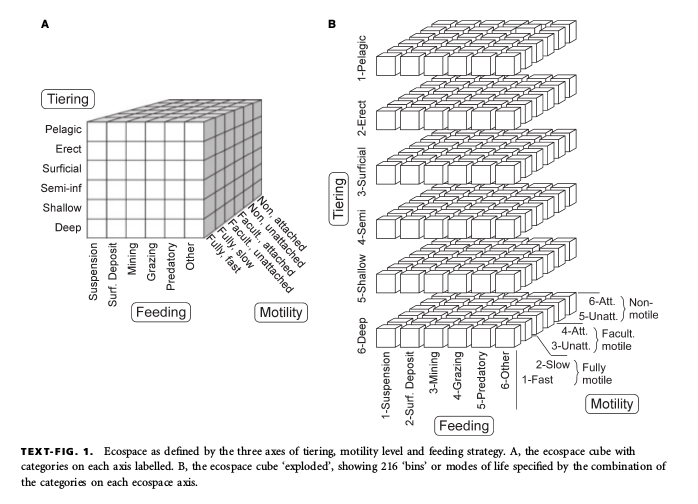
\includegraphics[height=0.8\textheight,width=\textwidth,keepaspectratio=true]{figure/ecocube}
  \end{center}

  \attrib{\footnotesize{Bambach \em{et al.}, 2007, \em{Palaeontology}}}
\end{frame}

\begin{frame}
  \frametitle{Fourth-corner modelling problem}
  \begin{center}
    %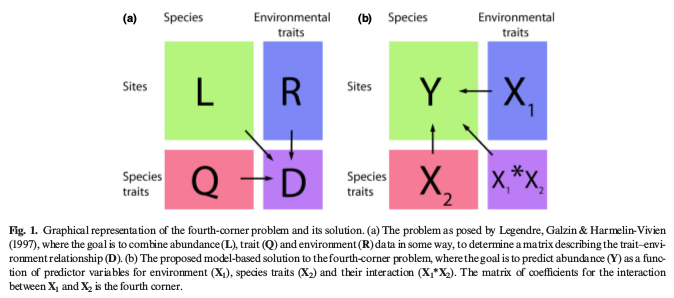
\includegraphics[height=0.8\textheight,width=\textwidth,keepaspectratio=true]{figure/warton_fourth_corner}
  \end{center}

  \attrib{\footnotesize{Brown \em{et al.}, 2014, \em{Methods Ecol. Evol.}}}
\end{frame}

\begin{frame}
  \frametitle{Covariates of interest}
  \begin{columns}
    \begin{column}{0.5\textwidth}
      individual-level \\(species i at time unit t)
      \begin{itemize}
        \item log-odds of occurrence probability at time t
        \item effect of locomotor type
          \begin{itemize}
            \item arboreal, digitigrade, plantigrade, unguligrade, fossorial, scansorial
          \end{itemize}
        \item effect of dietary type
          \begin{itemize}
            \item carnivore, herbivore, insectivore, omnivore
          \end{itemize}
        \item effect body size \\(rescaled log body mass)
      \end{itemize}
    \end{column}
    \begin{column}{0.5\textwidth}
      group-level (2 My time unit t)
      \begin{itemize}
        \item overall mean of log-odds of occurrence probability
        \item temperature record based on Mg/Ca estimates
          \begin{itemize}
            \item mean and interquartile range of rescaled value
          \end{itemize}
        \item plant community phase following Graham 2011
      \end{itemize}
    \end{column}
  \end{columns}
\end{frame}


%\begin{frame}
%  \frametitle{Model of taxon occurrence}
%  \begin{itemize}
%    \item response is p/a of genus in NA at time \(t\)
%      \begin{itemize}
%        \item Bernoulli variable 
%        \item probability is (observation prob) times (``true'' presence)
%      \end{itemize}
%    \item observation probability is effect of sampling/fossil record
%    \item the latent discrete ``true'' presence modeled as a \\multi-level logistic regression
%      \begin{itemize}
%        \item individual- and group-level covariates
%      \end{itemize}
%  \end{itemize}
%\end{frame}

\begin{frame}
  \frametitle{Paleontological fourth-corner model}
  \begin{center}
    %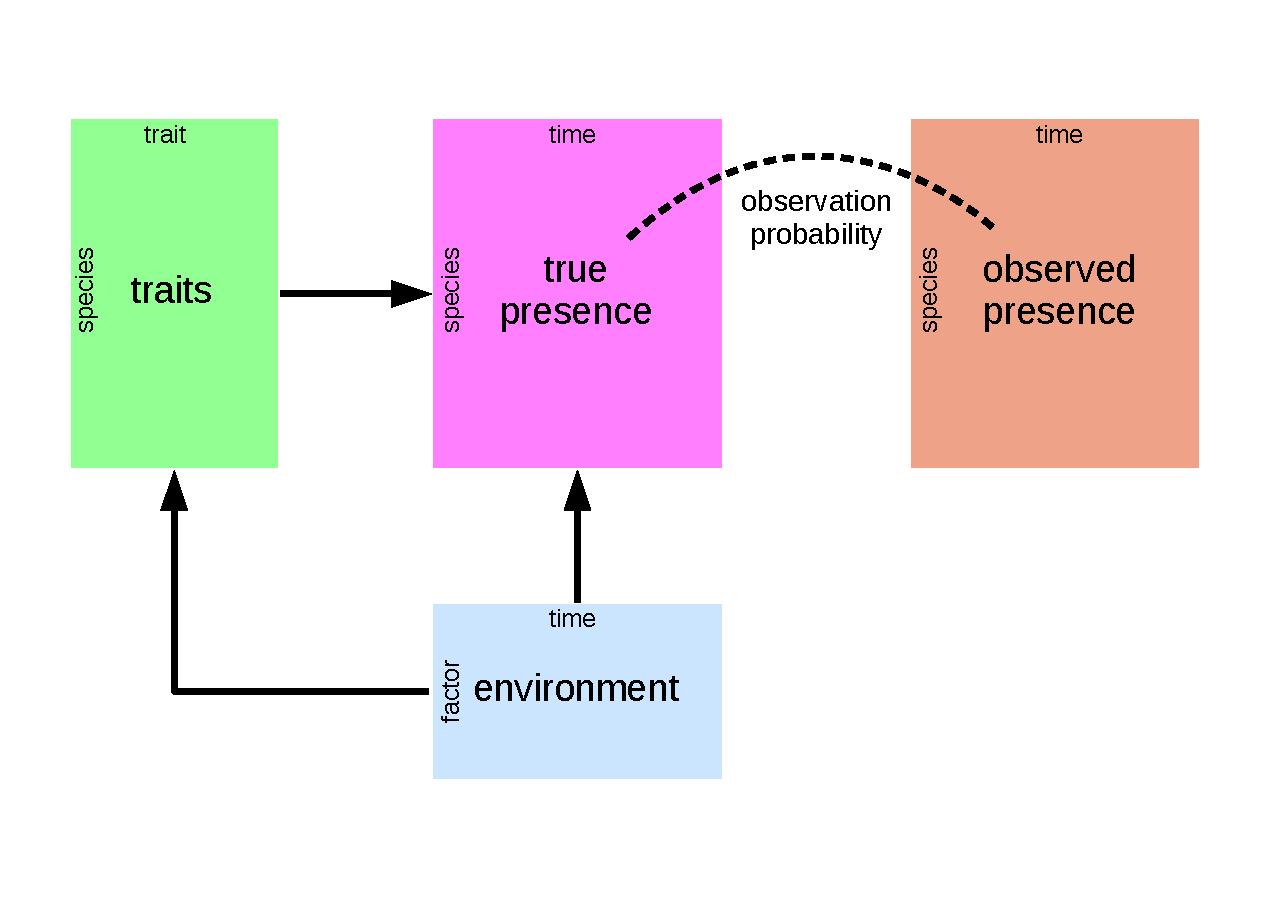
\includegraphics[height=0.8\textheight,width=\textwidth,keepaspectratio=true]{figure/paleo_fourth_corner}
  \end{center}

\end{frame}

\begin{frame}
  \frametitle{Model and sampling statement definition}
  \begin{footnotesize}
    \begin{columns}
      \begin{column}{0.5\textwidth}
        \begin{align*}
          y_{i, t} &\sim \text{Bernoulli}(p_{i, t} z_{i, t}) \\
          p_{i, t} &= \text{logit}^{-1}(\alpha_{0} + \alpha_{1} m_{i} + r_{t}) \\ 
          r_{t} &\sim \mathcal{N}(0, \sigma) \\
          \alpha_{0} &\sim \mathcal{N}(0, 1) \\
          \alpha_{1} &\sim \mathcal{N}(1, 1) \\
          \sigma &\sim \mathcal{N}^{+}(1) \\
          z_{i, 1} &\sim \text{Bernoulli}(\phi_{i, 1}) \\
          z_{i, t} &\sim \text{Bernoulli}\left(z_{i, t - 1} \pi_{i,t} + \sum_{x = 1}^{t}(1 - z_{i, x}) \phi_{i,t}\right) \\
          \phi_{i, t} &= \text{logit}^{-1}(a^{\phi}_{t, j[i]} + b^{\phi}_{1} m_{i} + b^{\phi}_{2} m_{i}^{2}) \\
          \pi_{i, t} &= \text{logit}^{-1}(a^{\pi}_{t, j[i]} + b^{\pi}_{1} m_{i} + b^{\pi}_{2} m_{i}^{2}) \\
          a^{\phi} &\sim \text{MVN}(U \gamma^{\phi}, \Sigma^{\phi}) \\
          a^{\pi} &\sim \text{MVN}(U \gamma^{\pi}, \Sigma^{\pi}) \\
        \end{align*}
      \end{column}
      \begin{column}{0.5\textwidth}
        \begin{align*}
          \Sigma^{\phi} &= \text{diag}(\tau^{\phi}) \Omega^{\phi} \text{diag}(\tau^{\phi}) \\
          \Sigma^{\pi} &= \text{diag}(\tau^{\pi}) \Omega^{\pi} \text{diag}(\tau^{\pi}) \\
          \rho &\sim \text{U}(0, 1) \\
          b^{\phi}_{1} &\sim \mathcal{N}(0, 1) \\
          b^{\pi}_{1} &\sim \mathcal{N}(0, 1) \\
          b^{\phi}_{2} &\sim \mathcal{N}(-1, 1) \\
          b^{\pi}_{2} &\sim \mathcal{N}(-1, 1) \\
          \gamma^{\phi} &\sim \mathcal{N}(0, 1) \\
          \gamma^{\pi} &\sim \mathcal{N}(0, 1) \\
          \tau^{\phi} &\sim \mathcal{N}^{+}(1) \\
          \tau^{\pi} &\sim \mathcal{N}^{+}(1) \\
          \Omega^{\phi} &\sim \text{LKJ}(2) \\
          \Omega^{\pi} &\sim \text{LKJ}(2). \\
        \end{align*}
      \end{column}
    \end{columns}
  \end{footnotesize} 


%  \scriptsize{Note: Product term ensures taxon-loss is permanent. Implementation in Stan marginalizes over all possible (range-through) values of \(z\) instead of estimating the discrete parameters. I also use a noncentered parameterization of the hierarchical effects for better posterior sampling behavior.} 
\end{frame}



\begin{frame}
  \frametitle{Posterior predictive performance}
\end{frame}

%\begin{frame}
%  \frametitle{Effect of mass on log-odds of observation}
%\end{frame}
%
%\begin{frame}
%  \frametitle{Effect of mass on log-odds of occurrence}
%\end{frame}

\begin{frame}
  \frametitle{Probability of ecotype origination}
\end{frame}

\begin{frame}
  \frametitle{Probability of ecotype survival}
\end{frame}

\begin{frame}
  \frametitle{Group-level effects (plant phase, climate)}
\end{frame}

\begin{frame}
  \frametitle{Total species pool diversity and diversification}
\end{frame}

\begin{frame}
  \frametitle{Ecotype-specific diversity}
\end{frame}

\begin{frame}
  \frametitle{Ecotype-specific origination}
\end{frame}

\begin{frame}
  \frametitle{Ecotype-specific extinction}
\end{frame}

\begin{frame}
  \begin{block}{Concerns and conclusions}
    \begin{itemize}
      \item basic and full models have similar results until Neogene
      \item posterior predictive simulations disimilar to observed; poor model adequacy
        \begin{itemize}
          \item previous work has \emph{never} evaluated model adequacy
          \item second-order Markov process?
          \item full posterior inference?
        \end{itemize}
      \item decreasing ability to discern arboreal taxa over time (absence/increased rarity)
      \item increase in scansorial taxa over time
      \item increase in herbivorous taxa over time
      \item plant phase has small, idiosyncratic effects
    \end{itemize}
  \end{block}
\end{frame}




\section{Conclusions and commentary}
\begin{frame}
  \frametitle{Summary}

  three studies on emergent patterns and their relation to functional traits

  many questions and hypotheses, both domain specific and general
\end{frame}

\begin{frame}
  \frametitle{Advances}

  law of constant extinction

  survival of the unspecialized

  functional diversity
\end{frame}

\begin{frame}
  \frametitle{Future}

  spatial data

  better models of preservation

  better hypotheses of relation between trait and target (ezard example)
\end{frame}

\begin{frame}
  \frametitle{Final thoughts}
\end{frame}





\appendix
%\begin{frame}
%  \begin{block}{New measure of taxon's environmental affinity}
%    (\# epicontinental / total \# occurrences) is what quantile of the distribution of all other background occurrences Beta(\(\alpha\), \(\beta\)).
%    \begin{itemize}
%      \item \(\alpha\) is the \# epicontinental background occurrences (+ 1).
%      \item \(\beta\) is the \# open ocean background (+ 1).
%    \end{itemize}
%  \end{block}
%\end{frame}
%
%
%\begin{frame}
%  \begin{block}{Measure of sampling and imputed values}
%    Sampling is measured as the gap statistic \(r\): \\(number of bins with an occurrence - 2) / (duration in bins - 2)
%
%    Can only be estimated for taxa with duration of three or more. \\Have to impute (e.g. fill-in) the values for all other taxa \(r^{\ast}\).
%    \begin{align*}
%      s &\sim \text{Beta}(\phi, \lambda) \\
%      \phi &= \text{logit}^{-1}(W\gamma) \\
%      s^{\ast} &\sim \text{Beta}(\phi^{\ast}, \lambda) \\
%      \phi^{\ast} &= \text{logit}^{-1}(W^{\ast}\gamma) \\
%    \end{align*}
%    \scriptsize{Note: Beta distribution parameterized in terms of mean \(\phi\) and total count \(\lambda\). \\Also, this presentation excludes final (hyper)priors.}
%  \end{block}
%\end{frame}

\end{document}
